\section[MIDI: An Introduction]{MIDI}\label{section:midi}

\subsection[What is MIDI?]{What is MIDI?}\label{section:what-midi}
The Musical Instrument Digital Interface (more commonly known as MIDI) is a digital communications protocol which allows for multiple hardware and software electronic instruments, controllers, computers, and related devices to communicate over a connected network\cite{Huber_2012}. It is used most to translate performance \say{events} (or musical notes) into its equivalent digital message, and then transmit these messages to other MIDI devices. These devices (MIDI receivers) can control sound generators or performance generators to create or modify music. Any MIDI-compatible device can send or receive MIDI messages from a MIDI controller (or the device sending the MIDI messages), and this will include all types of synthesizers. As an \say{interface}, MIDI is composed of a data communications link, and a system of hardware and software connected through this MIDI network. With MIDI, any electronic instruments and devices which are within a network can be worked with, through the transmission of a real-time performance and MIDI messages. These transmissions of performances and messages can then be put through the system to various instruments and devices through one singular data line, rather than multiple data streams, as this system can be chained from one device to another. A single data cable used with MIDI is capable of transmitting a real-time performance and MIDI-control message over 16 distinct channels, numbered appropriately one through sixteen. The musician working with the system will determine which of these channels to send information through, depending on which MIDI devices are being used\cite{Romano_2003}.

However, are several limitations to the MIDI protocol. The first, and most important, limitation of MIDI is that it does not support sound. It is unable to communicate audio itself, or create sounds\cite{Huber_2012}. Instead, as a digital language, it instructs a compatible device or program to create, playback, or modify sounds. It will communication an on/off status of a sound trigger, along with a range of parameters which instructs a MIDI receiver to control specified audio-related functions \cite{Kirk_Hunt_2013}. So, the data pathways for MIDI and audio routing will be different, even if they share a physical transmission cable, as in figure \ref{fig:midi-system-with-audio-connections}\cite{Huber_2012}. 

\begin{figure}
	\centering
	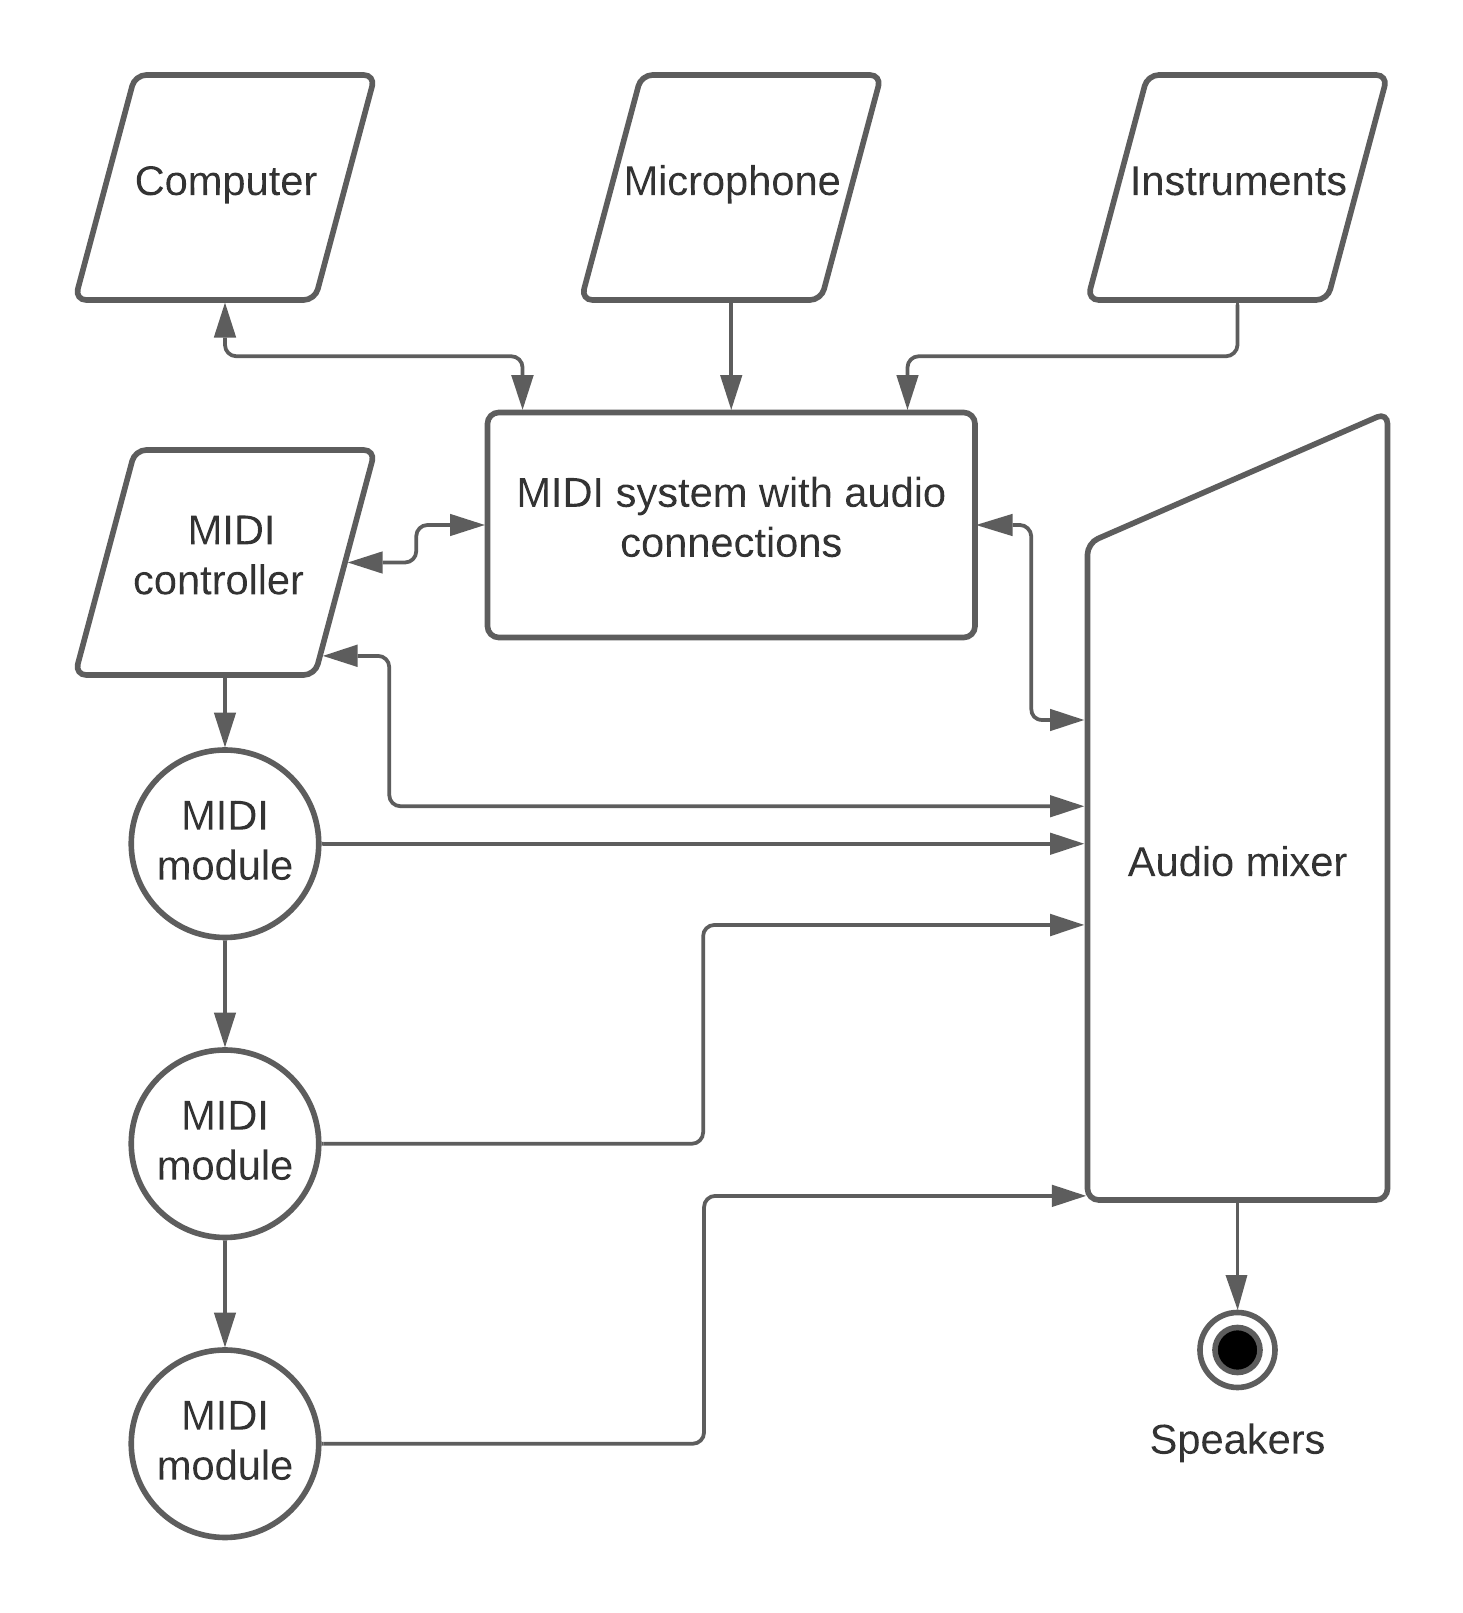
\includegraphics[width=0.35\textwidth]{figures/midi-system-with-audio-connections.png}
	\caption{The MIDI system, with audio connections}
	\label{fig:midi-system-with-audio-connections}
\end{figure}

Additionally, much of MIDI is built around the concept of keyboard notes and pitches. MIDI messages are primarily transmitted through the use of an electronic keyboard. So, for other types of MIDI instruments (such as a violin, or clarinet), there is a restriction to how a note may sound using MIDI. Certain characteristics of non-keyboard instruments (such as the ability of playing discrete semitone pitches) are more easily lost. For players of acoustic instruments, these issues are even more clear. Within MIDI, the velocity considered to be a single note-on velocity, defining the dynamic response of the note to one value. For players of acoustic instruments, the velocity, or dynamic response, of a singular note is shaped by the player, along with the note's timbre and pitch when played\cite{Kirk_Hunt_2013}.

\subsection[How does MIDI work?]{How does MIDI work?}\label{section:how-midi}
From a hardware perspective, the MIDI protocol will determine which types of plugs can be used for MIDI connections. There are three possible \say{sockets} that can be used on any MIDI-compatible device:

\begin{enumerate}
	\item MIDI OUT: this will send data to other devices (MIDI receivers). An example of this will include an electronic keyboard which plays a note, and then \say{note messages} are sent out from the MIDI OUT socket
	\item MIDI IN: this socket will receive the MIDI information from other devices. Using the previous example, if a keyboard's MIDI OUT socket is connected with a MIDI cable to another sound module's IN socket, then the sound module will be able to produce sound on behalf of the keyboard
	\item MIDI THRU: this socket will relay the messages received at the MIDI IN socket, so more devices will be able to be chained together.
\end{enumerate}\label{enu:list-of-midi-sockets}

\begin{figure}
	\centering
	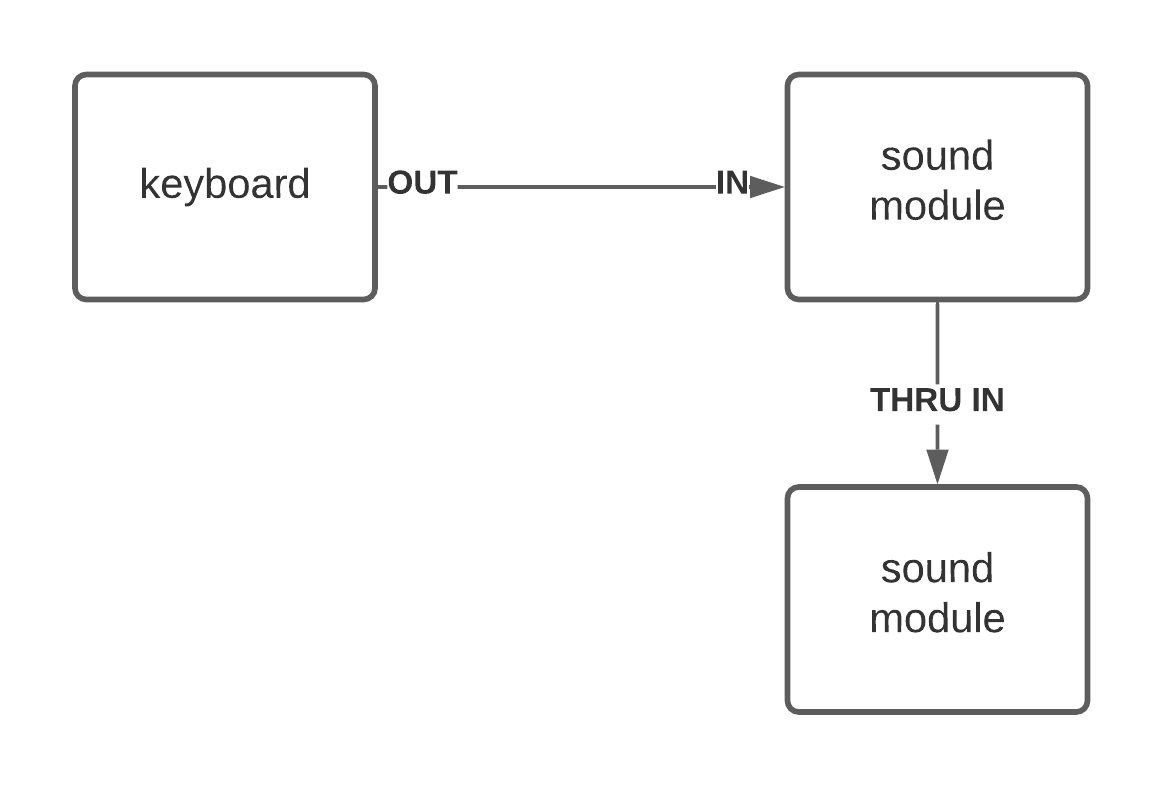
\includegraphics[width=0.5\textwidth]{figures/midi-sockets.png}
	\caption{MIDI sockets using an electronic keyboard}
	\label{fig:midi-sockets}
\end{figure}

Typically, this will result in the flow in figure \ref{fig:midi-sockets}, as it is normal for a keyboard's OUT port to be connected to a sound module's IN port. This IN socket will then be connected to another sound module, through the THRU IN port of the first sound module, into the IN port of the second sound module. Thus, both modules are now driven by the keyboard\cite{Kirk_Hunt_2013}.

In a software view of the protocol, there are two basic types of messages MIDI is able to send: a \textit{channel} message, and a \textit{system} message. Channel messages are much more common. As previously mentioned, MIDI allows for the use of up to 16 different sounds to be controlled at the same time, through the use of its 16 different channels. So, each sound that must be played concurrently will be placed into a different \textit{MIDI channel}. Within the channel, there are seven distinct messages, each of which contain a specific meaning and role. The first is the \say{Note on} message. This is the most common MIDI message used, and is sent whenever a note on a MIDI controller is played or pressed down, most common as pressing a key on a keyboard. The data contained in this message will tell a sound module how hard and fast a note was played (the \textit{velocity} of a note), as well as which channel the note was played on\cite{Romano_2003}. The pitch of the message represents which key was pressed, and is defined as the number for each semitone on a keyboard. Middle C ($C_4$) is number 60, and each semitone above and below Middle C is incremented or decremented accordingly\cite{Kirk_Hunt_2013}. The second is the \say{Note off} message, which turn off a note, or notes when a note is stopped. Like with Note on, Note off also contains values for channel, pitch, and velocity. For this message, only velocity's definition is changed, referring instead to the speed at which a note is released. The final common type of channel MIDI message is the \say{Pitch-bend}, which for electronic keyboard appears in the form of a physical wheel or sideways-moving handle of some type. Like its name implies, users will use this wheel or module to bend the pitch of notes currently being played. If the module is a physical wheel, it will return to its default position of zero (not bending a note) when the player lets go of the wheel. The pitch-bend will contain two pieces of data: the channel, and the pitch bend value. This value ranges from 0-127, with a value of 0 representing that the pitch has a full downwards bend to it, while a value of 127 represents the opposite, with a full upwards bend\cite{Kirk_Hunt_2013}. For this module, the value 64 will roughly indicate the center position on the wheel, and represent that a pitch has no bend applied to it.

MIDI also contains \say{system} messages, sent to all devices within the MIDI system. These messages are not limited to a specified number of channels, and allow for a greater variety of data to be sent. There are three basic types of system messages:

\begin{enumerate}
	\item real-time: this type of message allows the devices within the MIDI system to synchronize together
	\item common: this message allows the devices to agree on some type of common musical issues, with tuning and song selection as two examples
	\item exclusive: this message will exclusively send data to one device type. For manufacturers, these messages are used to send data to only one type of synthesizer or device type, serving as \say{add-ons} to MIDI.
\end{enumerate}\label{enu:midi-system-messages}

System messages are much harder to understand than channel messages, and so will not be discussed to great detail within the scope of this project.